% Options for packages loaded elsewhere
\PassOptionsToPackage{unicode}{hyperref}
\PassOptionsToPackage{hyphens}{url}
\PassOptionsToPackage{dvipsnames,svgnames,x11names}{xcolor}
%
\documentclass[
  10pt,
]{article}
\usepackage{amsmath,amssymb}
\usepackage{iftex}
\ifPDFTeX
  \usepackage[T1]{fontenc}
  \usepackage[utf8]{inputenc}
  \usepackage{textcomp} % provide euro and other symbols
\else % if luatex or xetex
  \usepackage{unicode-math} % this also loads fontspec
  \defaultfontfeatures{Scale=MatchLowercase}
  \defaultfontfeatures[\rmfamily]{Ligatures=TeX,Scale=1}
\fi
\usepackage{lmodern}
\ifPDFTeX\else
  % xetex/luatex font selection
  \setmainfont[]{Noto Serif}
  \setsansfont[]{Noto Sans}
  \setmonofont[]{DejaVu Sans Mono}
\fi
% Use upquote if available, for straight quotes in verbatim environments
\IfFileExists{upquote.sty}{\usepackage{upquote}}{}
\IfFileExists{microtype.sty}{% use microtype if available
  \usepackage[]{microtype}
  \UseMicrotypeSet[protrusion]{basicmath} % disable protrusion for tt fonts
}{}
\makeatletter
\@ifundefined{KOMAClassName}{% if non-KOMA class
  \IfFileExists{parskip.sty}{%
    \usepackage{parskip}
  }{% else
    \setlength{\parindent}{0pt}
    \setlength{\parskip}{6pt plus 2pt minus 1pt}}
}{% if KOMA class
  \KOMAoptions{parskip=half}}
\makeatother
\usepackage{xcolor}
\usepackage[margin=19mm]{geometry}
\usepackage{color}
\usepackage{fancyvrb}
\newcommand{\VerbBar}{|}
\newcommand{\VERB}{\Verb[commandchars=\\\{\}]}
\DefineVerbatimEnvironment{Highlighting}{Verbatim}{commandchars=\\\{\}}
% Add ',fontsize=\small' for more characters per line
\newenvironment{Shaded}{}{}
\newcommand{\AlertTok}[1]{\textcolor[rgb]{1.00,0.00,0.00}{\textbf{#1}}}
\newcommand{\AnnotationTok}[1]{\textcolor[rgb]{0.38,0.63,0.69}{\textbf{\textit{#1}}}}
\newcommand{\AttributeTok}[1]{\textcolor[rgb]{0.49,0.56,0.16}{#1}}
\newcommand{\BaseNTok}[1]{\textcolor[rgb]{0.25,0.63,0.44}{#1}}
\newcommand{\BuiltInTok}[1]{\textcolor[rgb]{0.00,0.50,0.00}{#1}}
\newcommand{\CharTok}[1]{\textcolor[rgb]{0.25,0.44,0.63}{#1}}
\newcommand{\CommentTok}[1]{\textcolor[rgb]{0.38,0.63,0.69}{\textit{#1}}}
\newcommand{\CommentVarTok}[1]{\textcolor[rgb]{0.38,0.63,0.69}{\textbf{\textit{#1}}}}
\newcommand{\ConstantTok}[1]{\textcolor[rgb]{0.53,0.00,0.00}{#1}}
\newcommand{\ControlFlowTok}[1]{\textcolor[rgb]{0.00,0.44,0.13}{\textbf{#1}}}
\newcommand{\DataTypeTok}[1]{\textcolor[rgb]{0.56,0.13,0.00}{#1}}
\newcommand{\DecValTok}[1]{\textcolor[rgb]{0.25,0.63,0.44}{#1}}
\newcommand{\DocumentationTok}[1]{\textcolor[rgb]{0.73,0.13,0.13}{\textit{#1}}}
\newcommand{\ErrorTok}[1]{\textcolor[rgb]{1.00,0.00,0.00}{\textbf{#1}}}
\newcommand{\ExtensionTok}[1]{#1}
\newcommand{\FloatTok}[1]{\textcolor[rgb]{0.25,0.63,0.44}{#1}}
\newcommand{\FunctionTok}[1]{\textcolor[rgb]{0.02,0.16,0.49}{#1}}
\newcommand{\ImportTok}[1]{\textcolor[rgb]{0.00,0.50,0.00}{\textbf{#1}}}
\newcommand{\InformationTok}[1]{\textcolor[rgb]{0.38,0.63,0.69}{\textbf{\textit{#1}}}}
\newcommand{\KeywordTok}[1]{\textcolor[rgb]{0.00,0.44,0.13}{\textbf{#1}}}
\newcommand{\NormalTok}[1]{#1}
\newcommand{\OperatorTok}[1]{\textcolor[rgb]{0.40,0.40,0.40}{#1}}
\newcommand{\OtherTok}[1]{\textcolor[rgb]{0.00,0.44,0.13}{#1}}
\newcommand{\PreprocessorTok}[1]{\textcolor[rgb]{0.74,0.48,0.00}{#1}}
\newcommand{\RegionMarkerTok}[1]{#1}
\newcommand{\SpecialCharTok}[1]{\textcolor[rgb]{0.25,0.44,0.63}{#1}}
\newcommand{\SpecialStringTok}[1]{\textcolor[rgb]{0.73,0.40,0.53}{#1}}
\newcommand{\StringTok}[1]{\textcolor[rgb]{0.25,0.44,0.63}{#1}}
\newcommand{\VariableTok}[1]{\textcolor[rgb]{0.10,0.09,0.49}{#1}}
\newcommand{\VerbatimStringTok}[1]{\textcolor[rgb]{0.25,0.44,0.63}{#1}}
\newcommand{\WarningTok}[1]{\textcolor[rgb]{0.38,0.63,0.69}{\textbf{\textit{#1}}}}
\usepackage{longtable,booktabs,array}
\usepackage{calc} % for calculating minipage widths
% Correct order of tables after \paragraph or \subparagraph
\usepackage{etoolbox}
\makeatletter
\patchcmd\longtable{\par}{\if@noskipsec\mbox{}\fi\par}{}{}
\makeatother
% Allow footnotes in longtable head/foot
\IfFileExists{footnotehyper.sty}{\usepackage{footnotehyper}}{\usepackage{footnote}}
\makesavenoteenv{longtable}
\usepackage{graphicx}
\makeatletter
\def\maxwidth{\ifdim\Gin@nat@width>\linewidth\linewidth\else\Gin@nat@width\fi}
\def\maxheight{\ifdim\Gin@nat@height>\textheight\textheight\else\Gin@nat@height\fi}
\makeatother
% Scale images if necessary, so that they will not overflow the page
% margins by default, and it is still possible to overwrite the defaults
% using explicit options in \includegraphics[width, height, ...]{}
\setkeys{Gin}{width=\maxwidth,height=\maxheight,keepaspectratio}
% Set default figure placement to htbp
\makeatletter
\def\fps@figure{htbp}
\makeatother
\setlength{\emergencystretch}{3em} % prevent overfull lines
\providecommand{\tightlist}{%
  \setlength{\itemsep}{0pt}\setlength{\parskip}{0pt}}
\setcounter{secnumdepth}{-\maxdimen} % remove section numbering
\ifLuaTeX
\usepackage[bidi=basic]{babel}
\else
\usepackage[bidi=default]{babel}
\fi
\babelprovide[main,import]{russian}
\ifPDFTeX
\else
\babelfont{rm}[]{Noto Serif}
\fi
% get rid of language-specific shorthands (see #6817):
\let\LanguageShortHands\languageshorthands
\def\languageshorthands#1{}
% Keep complete scientific figures together with their captions.
\usepackage{float}
\floatplacement{figure}{H}
% Long command lines should wrap within the text area.
\usepackage{fvextra}
\RecustomVerbatimEnvironment{Highlighting}{Verbatim}{commandchars=\\\{\},breaklines,breakanywhere}
\ifLuaTeX
  \usepackage{selnolig}  % disable illegal ligatures
\fi
\usepackage{bookmark}
\IfFileExists{xurl.sty}{\usepackage{xurl}}{} % add URL line breaks if available
\urlstyle{same}
\hypersetup{
  pdftitle={MD-A*: перенос, сравнение и оценка качества},
  pdfauthor={Исследовательский артефакт, ветка research/md-astar},
  pdflang={ru-RU},
  colorlinks=true,
  linkcolor={Maroon},
  filecolor={Maroon},
  citecolor={Blue},
  urlcolor={Blue},
  pdfcreator={LaTeX via pandoc}}

\title{MD-A*: перенос, сравнение и оценка качества}
\usepackage{etoolbox}
\makeatletter
\providecommand{\subtitle}[1]{% add subtitle to \maketitle
  \apptocmd{\@title}{\par {\large #1 \par}}{}{}
}
\makeatother
\subtitle{Нативный эксперимент в Incremental-MeshA/introduction}
\author{Исследовательский артефакт, ветка research/md-astar}
\date{Ноябрь 2026}

\begin{document}
\maketitle

\subsection{Аннотация}\label{ux430ux43dux43dux43eux442ux430ux446ux438ux44f}

В репозиторий перенесён MD-A* --- планировщик с сертификатом покрытой
клетки, ограниченной рабочей картой и очередью отложенных освобождений.
Реализация написана на Python и использует исходные car16,
float-стоимости и карты проекта. Она сравнивается со всеми шестью
основными алгоритмами репозитория и с тем же MPGAA*, который служит её
базовым поиском. Ускорение MD-A* относительно MPGAA*: исходные задачи
--- 0.98 {[}0.97; 1.00{]}×; смешанные обновления --- 1.02 {[}0.99;
1.02{]}×; новый seed --- 1.00×; диагностическая семья --- 144.08×. На 40
эпизодах (280 записях «эпизод, запрос») выполнено 1032 запусков и 7656
измеренных вызовов. Независимый Дейкстра проверил 1458 ответов; оба
новых планировщика дополнительно проверены на всех 561 исходных
запросах. Выводы о выгоде оболочки отделены от преимуществ самого
MPGAA*, а прежние C++-времена не используются.

\subsection{1. Что именно
добавлено}\label{ux447ux442ux43e-ux438ux43cux435ux43dux43dux43e-ux434ux43eux431ux430ux432ux43bux435ux43dux43e}

Новая ветка основана на актуальной default-ветке репозитория, commit
\texttt{cc58898}. \texttt{mesha/deferred.py} реализует MD-A*,
\texttt{mesha/adaptive.py} --- независимый порт MPGAA* (Hernández, Asín,
Baier, AAAI 2015, алгоритмы 1--2). Порт использует явных
предшественников ориентированных примитивов, группировку swept-cell
зависимостей и консервативную рамку всех когда-либо раскрытых
источников. Оболочка и отдельный MPGAA*-контроль используют \textbf{один
класс}, поэтому их прямое сравнение выделяет новый механизм.

MD-A* сохраняет фактическую карту и рабочий подграф. Освобождённая
клетка может оставаться занятой в рабочей карте, пока не способна
улучшить известный допустимый путь. При повреждении маршрута верхняя
граница растёт, и старые исключения пересматриваются. При неизвестной
достижимости включаются все отложенные клетки. Математически достаточно
нуля, одного или двух вызовов базового точного поиска. Состояния цели
фиксированы на протяжении эпизода.

Это поиск по \textbf{граничным состояниям mesh с полными примитивами как
макрорёбрами}. Внутренний mesh компилирует сертификат. MD-A* не
поддерживает метки всех регулярных расширенных клеток, как исходный D*
Lite (mesh). Эти два подхода решают одну дискретную задачу, но выполняют
раскрытия разного типа.

Добавлен API \texttt{replan(start,\ new\_blocks,\ new\_opens=())}. В D*
Lite при открытиях сбрасывается кеш затронутых рёбер и обновляются также
ранее неизвестные источники: ограничение лишь вершинами g/rhs было
безопасно для увеличений, но пропускало бы восстановление связности. Для
увеличений прежний фильтр сохранён. Дополнительные флаги
\texttt{search()} исключают визуализационные списки раскрытий и полную
трассу, сохраняя возврат состояний и примитивов. Старые вызовы и
значения по умолчанию совместимы. Исходные данные и опубликованные
результаты репозитория сохранены.

\subsection{2. Сертификат и
корректность}\label{ux441ux435ux440ux442ux438ux444ux438ux43aux430ux442-ux438-ux43aux43eux440ux440ux435ux43aux442ux43dux43eux441ux442ux44c}

Для примитива p со стоимостью \(C_p\), смещением \(\Delta_p\) и
покрытыми клетками \(T_p\) выбираем октильную норму \(D=\alpha d_8\)
так, чтобы \(D(0,\Delta_p)\le C_p\). Поправка и нижняя оценка имеют вид

\[m=\min_{p,d\in T_p}[C_p-D(0,d)-D(0,\Delta_p-d)],\qquad L_q(s,t)=D(s,q)+D(q,t)+m.\]

Два неравенства треугольника показывают: любой путь, покрывающий q,
стоит не меньше \(L_q\). Поправка необходима: кривая покрывает клетку,
не обязательно проходя через её центр. Норма представляется максимумом
восьми опорных функций; 64 префиксно-суффиксных коэффициента считаются
топологическими проходами DAG одного примитива. Терминальные рёбра
направляются в отдельные стоки, а не в следующий примитив. Основной
запрос использует один скаляр m; MD-64 --- усиленную оценку из 64 чисел.
Скаляр m можно получить и прямым перебором примитивов: необходимость
mesh для самой допустимости этой оценки не заявляется.

Если все ещё скрытые свободные клетки имеют \(L_q\ge U\), оптимальный
рабочий путь стоимости U оптимален фактически: более дешёвый путь либо
содержался бы в рабочем графе, либо покрывал бы исключённую клетку. При
допустимом старом суффиксе включаем потенциально полезные клетки и его
собственные скрытые клетки, затем достаточно одного поиска. Если
суффикса нет, первый рабочий поиск даёт \(U_0\); после включения клеток
с \(L_q<U_0\) второй поиск даёт \(U_1\le U_0\), так что остальные
исключения остаются верными. При \(U_0=\infty\) включаются все.

Чтобы не пересматривать историю при каждом движении, храним ключ
\(k_q=L_q(s_i,t)+A_i\), где A --- накопленная сумма геометрических
перемещений старта. Липшицевость \(|L_q(s,t)-L_q(s',t)|\le D(s,s')\)
даёт \(k_q-A_j\le L_q(s_j,t)\). Достаточно извлекать и уточнять ключи
ниже порога \(U+A_j\). Возврат старта назад безопасен; может возрасти
только работа уточнения.

В нативной модели 284 примитива и 412 конфигураций;
\(\alpha=0.926209683\), \(m\approx-0.438205819\). Стоимости не
квантуются. Сравнения консервативны относительно EPS проекта; совпадение
ответов проверяется с допуском \(10^{-6}\). Теорема дана для идеальной
арифметики; float-код не выдаётся за формально верифицированный
численный сертификат. Полное доказательство и численные оговорки:
\url{method.md}.

\subsection{3. Протокол
сравнения}\label{ux43fux440ux43eux442ux43eux43aux43eux43b-ux441ux440ux430ux432ux43dux435ux43dux438ux44f}

Сравниваются LBA*, LazyLBA*, MeshA*, Mesh/ParallA*, D* Lite на решётке и
mesh-графе, MPGAA* и MD-A*. Все реализации --- Python, все используют
одинаковый \texttt{car16}, стоимость и supercover. Вес равен 1.
Mesh/ParallA* имеет мягкое отсечение дубликатов и остаётся приближённым
контролем; его скорость не считается выигрышем точного поиска без учёта
стоимости.

Чистый Mesh/PruningA* --- неполный подалгоритм Mesh/ParallA*, а не
отдельный точный контроль. Взвешенные варианты w\textgreater1 в этой
фазе не измеряются.

Исходный набор --- 24 эпизода: по шести квантилям длины пар клеток на
каждой из четырёх карт (Berlin\_2\_256, AR0700SR, maze, rooms). Одна
пара курсов из каждой группы выбирается по детерминированной чётности
карты/страты. Выбор зафиксирован до времён MD-A*. Каждый эпизод содержит
три запроса, два из которых гарантированно ломают маршрут. Для
корректности используется весь исходный набор из 187 эпизодов, а не
только временная выборка.

Дополнение: восемь смешанных эпизодов на тех же четырёх картах
(фиксированный старт и возвраты), по 13 запросов, seed 761116. Квадрат
3×3 перемещается, освобождая старые клетки; раз в четыре события он
размещается на текущем контрольном пути. Четыре эпизода с seed 761117
проверяют перенос на новые запросы той же коллекции карт. Непроходимые
снимки не отбрасываются. Движение задаётся контрольным поиском, а не
кандидатом.

Диагностика --- четыре эпизода на пустых картах 80×80 и 160×160:
диагональный запрос, удалённые перемещения квадрата внутри большой рамки
поискового состояния, неподвижный или возвращающийся старт. Семья
выбрана для проверки механизма и не является оценкой среднего выигрыша
на произвольной карте.

\begin{longtable}[]{@{}lllll@{}}
\toprule\noalign{}
Набор & Эпизоды & Записи запросов & Строгий рост & Недостижимость \\
\midrule\noalign{}
\endhead
\bottomrule\noalign{}
\endlastfoot
Исходные & 24 & 72 & 48 & 0 \\
Смешанные & 8 & 104 & 20 & 2 \\
Новый seed & 4 & 52 & 11 & 0 \\
Диагностика & 4 & 52 & 0 & 0 \\
\end{longtable}

Среда: Python 3.12.14, NumPy 2.3.5, AMD EPYC 9V74 80-Core Processor. Три
повторения, последовательно, порядок методов перемешан для каждого
эпизода. Таймер включает применение изменений, поиск и извлечение
состояний/примитивов. Независимая проверка пути находится за таймером и
не прогревает кеши планировщика. Счётчики и стоимости должны совпадать
между повторениями. Общая неизменяемая модель готовится заранее, как в
проекте; конструкторы планировщиков измерены отдельно. Компилятор
сертификата потребовал 8.25 мс; дополнительно приводится консервативная
метрика, добавляющая эту цену один раз на эпизод MD-A*.

Метрика ускорения: отношение времени контроля к времени кандидата.
Сначала суммируем нужные запросы эпизода, затем берём медиану трёх
повторений и медиану парных отношений по эпизодам. Интервалы ---
описательная 95\% перевыборка четырёх кластеров-карт (6000 выборок), не
предположение независимости запросов. На новом seed и диагностической
семье интервалы не приводятся. Снимки означают записи «эпизод, запрос»;
некоторые парные эпизоды имеют совпадающие начальные запросы.

В первом проходе обнаружилось, что D* Lite применял прежний лимит 3 млн
раскрытий накопительно к 13 запросам. Протокол исправлен на 3 млн на
запрос. Сохранены только 21 целиком законченный эпизод, в котором
прежний ограничитель никогда не срабатывал; все неполные эпизоды
повторены целиком. В одной паре не смешиваются фазы. Точный diff
подтверждает, что изменилось только присваивание ограничителя вне
таймера; код алгоритмов и среда не менялись. Исходный проход, журнал
отказа и все его исходники сохранены в
\texttt{development/cumulative-budget-v1}, а IDs фаз --- в environment и
CSV.

\subsection{4. Измеренные
результаты}\label{ux438ux437ux43cux435ux440ux435ux43dux43dux44bux435-ux440ux435ux437ux443ux43bux44cux442ux430ux442ux44b}

\subsubsection{4.1. Все алгоритмы
репозитория}\label{ux432ux441ux435-ux430ux43bux433ux43eux440ux438ux442ux43cux44b-ux440ux435ux43fux43eux437ux438ux442ux43eux440ux438ux44f}

\begin{longtable}[]{@{}
  >{\raggedright\arraybackslash}p{(\columnwidth - 8\tabcolsep) * \real{0.2000}}
  >{\raggedright\arraybackslash}p{(\columnwidth - 8\tabcolsep) * \real{0.2000}}
  >{\raggedright\arraybackslash}p{(\columnwidth - 8\tabcolsep) * \real{0.2000}}
  >{\raggedright\arraybackslash}p{(\columnwidth - 8\tabcolsep) * \real{0.2000}}
  >{\raggedright\arraybackslash}p{(\columnwidth - 8\tabcolsep) * \real{0.2000}}@{}}
\toprule\noalign{}
\begin{minipage}[b]{\linewidth}\raggedright
Метод
\end{minipage} & \begin{minipage}[b]{\linewidth}\raggedright
Исходные, онлайн
\end{minipage} & \begin{minipage}[b]{\linewidth}\raggedright
Исходные, эпизод
\end{minipage} & \begin{minipage}[b]{\linewidth}\raggedright
Смешанные, онлайн
\end{minipage} & \begin{minipage}[b]{\linewidth}\raggedright
Макс. цена / оптимум
\end{minipage} \\
\midrule\noalign{}
\endhead
\bottomrule\noalign{}
\endlastfoot
LBA* & 1.00 {[}1.00; 1.00{]} & 1.00 {[}1.00; 1.00{]} & 1.00 {[}1.00;
1.00{]} & 1.0000 \\
LazyLBA* & 0.68 {[}0.57; 0.88{]} & 0.60 {[}0.53; 0.75{]} & 0.68 {[}0.50;
0.87{]} & 1.0000 \\
MeshA* & 0.49 {[}0.41; 0.50{]} & 0.40 {[}0.37; 0.48{]} & 0.37 {[}0.32;
0.64{]} & 1.0000 \\
Mesh/ParallA* & 0.59 {[}0.51; 0.81{]} & 0.58 {[}0.52; 0.74{]} & 0.12
{[}0.01; 0.43{]} & 2.3596 \\
D* Lite lattice & 0.36 {[}0.28; 1.15{]} & 0.42 {[}0.37; 0.61{]} & 1.09
{[}0.15; 3.13{]} & 1.0000 \\
D* Lite mesh & 0.13 {[}0.07; 0.44{]} & 0.09 {[}0.07; 0.21{]} & 0.13
{[}0.02; 1.61{]} & 1.0000 \\
MPGAA* & 0.73 {[}0.62; 1.50{]} & 0.71 {[}0.64; 0.78{]} & 5.58 {[}3.71;
6.45{]} & 1.0000 \\
MD-A* & 0.77 {[}0.61; 1.43{]} & 0.70 {[}0.64; 0.80{]} & 5.50 {[}3.83;
6.33{]} & 1.0000 \\
\end{longtable}

Ускорения этой таблицы --- к LBA* в той же новой серии; больше единицы
означает быстрее.

На исходном наборе MD-A* имеет ускорение 0.77× к LBA*: в этой метрике он
уступает простому повторному поиску. Прямое парное сравнение с D* Lite
(mesh) даёт 5.66 {[}3.82; 12.44{]}×. Различие этих выводов показывает,
почему сравнения только с D* Lite недостаточно.

\begin{figure}
\centering
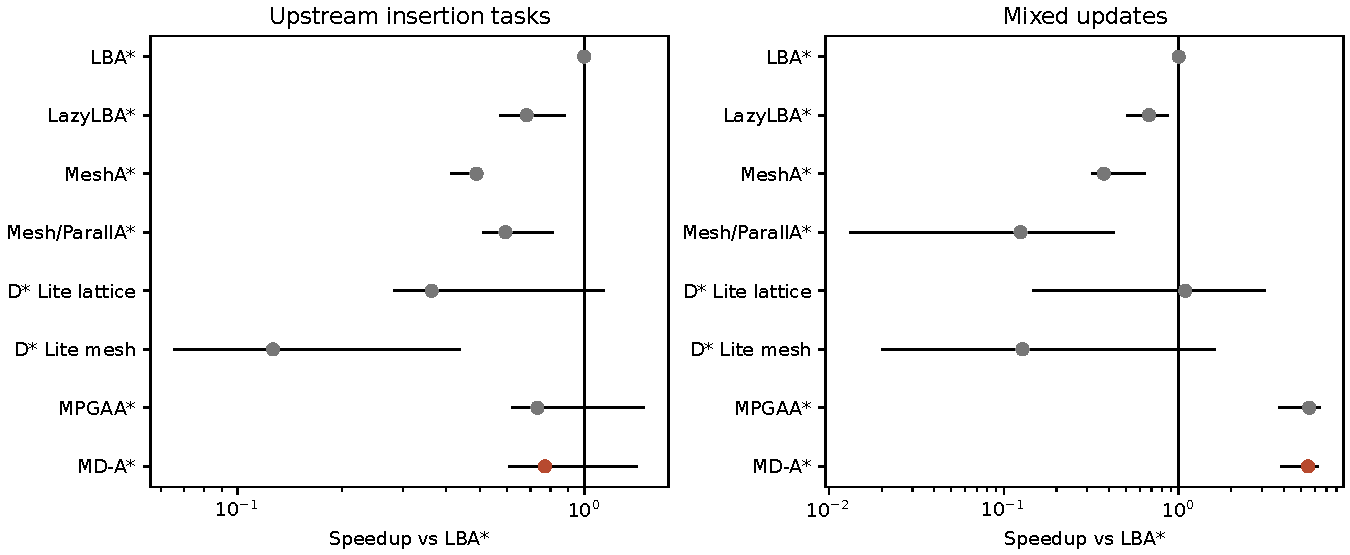
\includegraphics[width=0.98\textwidth,height=\textheight]{figures/comparison.pdf}
\caption{Нативные времена относительно LBA*. Серые контроли и MD-A*
используют один язык; интервалы сохраняют зависимость внутри карты.}
\end{figure}

\subsubsection{4.2. Выделение вклада
MD-A*}\label{ux432ux44bux434ux435ux43bux435ux43dux438ux435-ux432ux43aux43bux430ux434ux430-md-a}

\begin{longtable}[]{@{}
  >{\raggedright\arraybackslash}p{(\columnwidth - 10\tabcolsep) * \real{0.1667}}
  >{\raggedright\arraybackslash}p{(\columnwidth - 10\tabcolsep) * \real{0.1667}}
  >{\raggedright\arraybackslash}p{(\columnwidth - 10\tabcolsep) * \real{0.1667}}
  >{\raggedright\arraybackslash}p{(\columnwidth - 10\tabcolsep) * \real{0.1667}}
  >{\raggedright\arraybackslash}p{(\columnwidth - 10\tabcolsep) * \real{0.1667}}
  >{\raggedright\arraybackslash}p{(\columnwidth - 10\tabcolsep) * \real{0.1667}}@{}}
\toprule\noalign{}
\begin{minipage}[b]{\linewidth}\raggedright
Набор
\end{minipage} & \begin{minipage}[b]{\linewidth}\raggedright
Онлайн
\end{minipage} & \begin{minipage}[b]{\linewidth}\raggedright
Выигрыши
\end{minipage} & \begin{minipage}[b]{\linewidth}\raggedright
С конструктором
\end{minipage} & \begin{minipage}[b]{\linewidth}\raggedright
+ компилятор
\end{minipage} & \begin{minipage}[b]{\linewidth}\raggedright
Строгий рост
\end{minipage} \\
\midrule\noalign{}
\endhead
\bottomrule\noalign{}
\endlastfoot
Исходные & 0.98 {[}0.97; 1.00{]} & 10/24 & 0.99 {[}0.98; 1.00{]} & 0.96
{[}0.94; 0.96{]} & 0.98 {[}0.97; 1.00{]} \\
Смешанные & 1.02 {[}0.99; 1.02{]} & 5/8 & 1.01 {[}0.97; 1.01{]} & 0.97
{[}0.89; 0.99{]} & 0.98 {[}0.95; 1.00{]} \\
Новый seed & 1.00 & 2/4 & 1.03 & 0.98 & 1.01 \\
Диагностика & 144.08 & 4/4 & 12.38 & 3.65 & --- \\
\end{longtable}

Ускорение MD-A* относительно MPGAA*: время MPGAA*, делённое на время
MD-A*; больше единицы означает выигрыш MD-A*.

На исходных задачах интервал включает единицу; устойчивое общее
ускорение оболочки не установлено.

На смешанных задачах интервал включает единицу; устойчивое общее
ускорение оболочки не установлено.

Ускорение против D* Lite или MeshA* нельзя полностью приписать новому
сертификату: оно включает различия алгоритма ядра, направления поиска и
представления состояний. Именно прямая пара с общим MPGAA* является
причинным контролем.

На смешанном наборе 41.7\% перепланирований не вызывают ядро, однако
общий выигрыш близок к единице: в суммах времени доминируют дорогие
ремонты. Число пропущенных поисков само по себе не является достаточным
показателем ускорения.

\begin{figure}
\centering
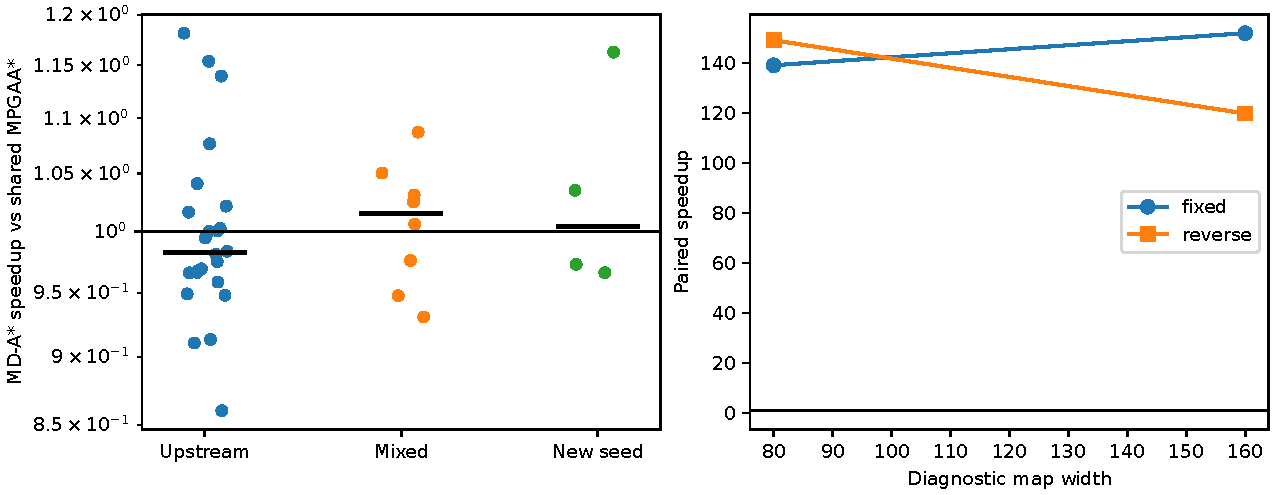
\includegraphics[width=0.98\textwidth,height=\textheight]{figures/transfer.pdf}
\caption{Ускорение MD-A* относительно MPGAA*: исходные задачи, смешанные
изменения, новый seed; отдельно параметрическая диагностика.}
\end{figure}

\subsubsection{4.3. Абляции и выполненная
работа}\label{ux430ux431ux43bux44fux446ux438ux438-ux438-ux432ux44bux43fux43eux43bux43dux435ux43dux43dux430ux44f-ux440ux430ux431ux43eux442ux430}

\begin{longtable}[]{@{}llllll@{}}
\toprule\noalign{}
Набор & Вариант & К LBA* & Без поиска & Два вызова & p95, мс \\
\midrule\noalign{}
\endhead
\bottomrule\noalign{}
\endlastfoot
Смешанные & MD-A* & 5.50 {[}3.83; 6.33{]} & 41.7\% & 15.6\% & 169.28 \\
Смешанные & MD-64 & 4.98 {[}3.37; 6.18{]} & 41.7\% & 15.6\% & 182.14 \\
Смешанные & MD scan & 4.85 {[}3.87; 6.68{]} & 41.7\% & 15.6\% &
162.06 \\
Диагностика & MD-A* & 92.89 & 100.0\% & 0.0\% & 0.04 \\
Диагностика & MD-64 & 15.47 & 100.0\% & 0.0\% & 0.21 \\
Диагностика & MD scan & 45.28 & 100.0\% & 0.0\% & 0.08 \\
\end{longtable}

MD-64 усиливает только оценку; MD scan заменяет только переносимую кучу
полным просмотром. p95 --- описание задержек, не интервал среднего
эффекта.

На диагностике простая скалярная версия быстрее MD-64 в 6.78 раза, а
варианта с полным просмотром --- в 2.21 раза по прямым парным
отношениям. Это поддерживает выбор простой версии для проверенного
режима, а не усложнение оценки.

\begin{figure}
\centering
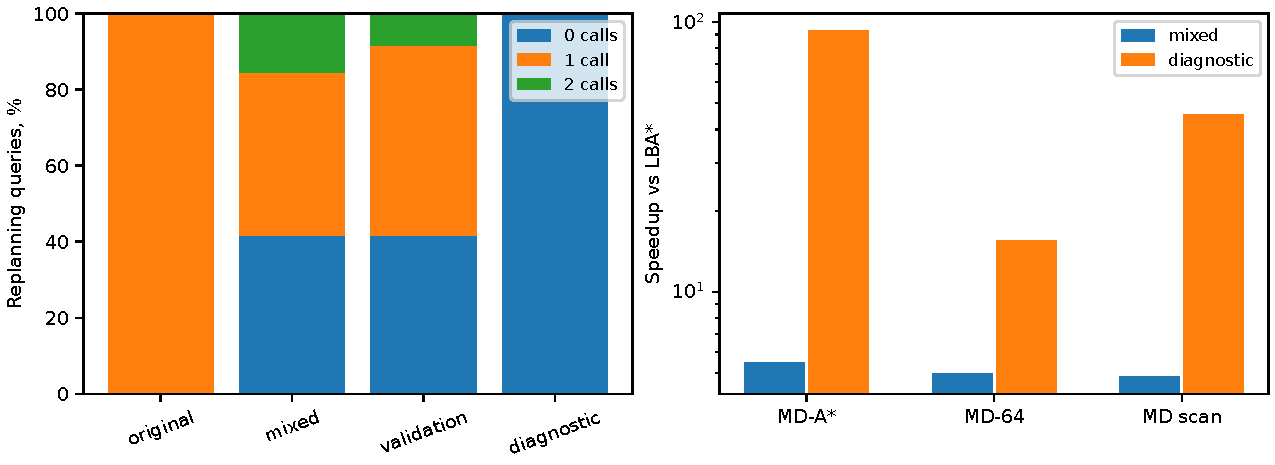
\includegraphics[width=0.98\textwidth,height=\textheight]{figures/mechanism.pdf}
\caption{Доля нуля, одного и двух вызовов ядра; цена усложнения
сертификата и полного просмотра истории.}
\end{figure}

\begin{longtable}[]{@{}lllll@{}}
\toprule\noalign{}
Набор & Метод & Раскрытия & Чтения клеток & Группы уведомлений \\
\midrule\noalign{}
\endhead
\bottomrule\noalign{}
\endlastfoot
Исходные & LBA* & 5025 & 193423 & --- \\
Исходные & D* Lite mesh & 12848 & 5217 & --- \\
Исходные & MPGAA* & 2731 & 59269 & 18564 \\
Исходные & MD-A* & 2731 & 59269 & 18564 \\
Смешанные & LBA* & 84543 & 2374595 & --- \\
Смешанные & D* Lite mesh & 1167084 & 108929 & --- \\
Смешанные & MPGAA* & 15534 & 178155 & 26928 \\
Смешанные & MD-A* & 15535 & 178168 & 25092 \\
Диагностика & LBA* & 1137 & 108015 & --- \\
Диагностика & D* Lite mesh & 0 & 64230 & --- \\
Диагностика & MPGAA* & 0 & 0 & 84456 \\
Диагностика & MD-A* & 0 & 0 & 0 \\
\end{longtable}

Это медианы сумм по перепланированиям эпизода. Раскрытие внутренней
mesh-конфигурации и граничного состояния решётки --- разные операции; их
отношение не считается универсальной мерой работы. Кеши могут дать ноль
новых чтений, но подготовка уведомлений всё равно стоить времени. У
MPGAA*/MD-A* раскрытия относятся к прямому A*, не включают извлечения
очереди ремонта эвристики; D* Lite считает свою очередь ремонта. Это
неполный профиль работы, а не взаимозаменяемые единицы. Счётчики
объясняют механизм, но не заменяют время.

\subsection{5. Корректность и
воспроизводимость}\label{ux43aux43eux440ux440ux435ux43aux442ux43dux43eux441ux442ux44c-ux438-ux432ux43eux441ux43fux440ux43eux438ux437ux432ux43eux434ux438ux43cux43eux441ux442ux44c}

Независимый Дейкстра проверил 308 снимков и 1458 ответов: car16 и
legacy8, все курсы, разрез и повторное соединение компонент, повторные
правки, блокировка концов для новых планировщиков, возвраты старта и 160
обновлений для очистки старых элементов кучи. Важный тест: стоимости
\(13 \to 13 \to 19\) при рабочем обходе 23 и реактивации старого
открытия; проверены именно два вызова MPGAA*. Все коэффициенты сверены с
прямым перебором, для каждого набора проверено 128 случайных
геометрических троек.

На всех 187 исходных эпизодах оба новых планировщика дали 1122
совпадающих со старым точным LBA* ответов и столько же допустимых
траекторий. Здесь старые записи используются только как стоимостной
эталон. Исходный selfcheck проекта также прошёл. В измерительной фазе
каждый возвращённый путь дополнительно проверен по всем покрытым клеткам
и конечному курсу; точные методы совпали с контрольной стоимостью.
Приближённый Mesh/ParallA* оценивается отдельно.

\subsection{6. Оценка качества проделанной
работы}\label{ux43eux446ux435ux43dux43aux430-ux43aux430ux447ux435ux441ux442ux432ux430-ux43fux440ux43eux434ux435ux43bux430ux43dux43dux43eux439-ux440ux430ux431ux43eux442ux44b}

\begin{longtable}[]{@{}
  >{\raggedright\arraybackslash}p{(\columnwidth - 4\tabcolsep) * \real{0.3333}}
  >{\raggedright\arraybackslash}p{(\columnwidth - 4\tabcolsep) * \real{0.3333}}
  >{\raggedright\arraybackslash}p{(\columnwidth - 4\tabcolsep) * \real{0.3333}}@{}}
\toprule\noalign{}
\begin{minipage}[b]{\linewidth}\raggedright
Критерий
\end{minipage} & \begin{minipage}[b]{\linewidth}\raggedright
Оценка
\end{minipage} & \begin{minipage}[b]{\linewidth}\raggedright
Основание
\end{minipage} \\
\midrule\noalign{}
\endhead
\bottomrule\noalign{}
\endlastfoot
Интеграция & Хорошая & Нативные структуры и API, общий MPGAA*-контроль,
исходные данные сохранены. \\
Корректность & Сильная экспериментальная проверка & Независимый
Dijkstra, все исходные запросы, каждая возвращённая траектория,
отдельное математическое доказательство. \\
Сопоставимость & Контролируется протоколом & Один язык, одни стоимости,
новые последовательные времена; нет сравнения C++ с Python или старых
секунд с новыми. \\
Новизна & Конкретная гипотеза, внешний приоритет не подтверждён &
Mesh-компиляция клеточного сертификата и переносимая очередь известного
уменьшения; сам A*/MPGAA*/кеш пути известны. \\
Общее преимущество & Определяется результатами раздела 4 & Целевой режим
нельзя переносить на гарантированные поломки маршрута. \\
Готовность к ведущей конференции & Исследовательский артефакт, не
готовая SOTA-заявка & Четыре основные карты, один основной control set,
временная выборка 24 исходных эпизодов и небольшой новый seed. \\
\end{longtable}

\textbf{Связь с предыдущим C++-артефактом.} Предыдущая C++-работа
использовала другие примитивы, целые стоимости и другие нагрузки. Её
112× относятся к специально выделенной диагностике, а не к исходным
задачам этого репозитория. Они сохранены в
\href{reference/README.md}{справочном артефакте}, но не выданы за
нативное воспроизведение. Новый набор отделяет проверку всего корпуса от
дорогого временного поднабора и не раздувает число независимых задач
повторениями/алгоритмами.

\textbf{Ограничения остаются.} Исходная постановка --- только добавление
препятствий на маршруте. В ней идея отсрочки освобождений почти не
используется; расширенная смешанная задача является отдельным
экспериментом. Для публикации нужны более широкие карты и control set,
длинные серии, сравнение с DPA*/L-GLS и независимыми оптимизированными
реализациями, раздельные абляции рабочего графа и самого сертификата,
более сильная численная гарантия. Коллизии здесь --- дешёвые чтения
2D-сетки точечного агента, а не измерение реального контура/3D. Пиковая
память не измерялась; дополнительная рабочая карта и история
освобождений требуют памяти. Цель фиксирована. При разрушении маршрута
два базовых поиска могут быть дороже одного; история перемещений может
ослабить ключи и потребовать массового уточнения.

Работу стоит оценивать как воспроизводимый и проверяемый алгоритмический
эксперимент с обоснованным механизмом, а не как доказанное универсальное
превосходство. Практический выбор должен опираться на частоту
несущественных изменений и цену действительного обхода.

\subsection{7.
Воспроизведение}\label{ux432ux43eux441ux43fux440ux43eux438ux437ux432ux435ux434ux435ux43dux438ux435}

\begin{Shaded}
\begin{Highlighting}[]
\ExtensionTok{pip}\NormalTok{ install }\AttributeTok{{-}r}\NormalTok{ requirements{-}md{-}astar.txt}
\ExtensionTok{python} \AttributeTok{{-}m}\NormalTok{ mesha.selfcheck}
\ExtensionTok{python} \AttributeTok{{-}m}\NormalTok{ mesha.selfcheck\_deferred}
\ExtensionTok{python} \AttributeTok{{-}m}\NormalTok{ mesha.validate\_md\_suite}
\ExtensionTok{python} \AttributeTok{{-}m}\NormalTok{ mesha.md\_benchmark }\AttributeTok{{-}{-}run} \AttributeTok{{-}{-}cohort}\NormalTok{ all}
\ExtensionTok{python}\NormalTok{ tools\_md\_analyze.py}
\ExtensionTok{python}\NormalTok{ tools\_md\_report.py }\AttributeTok{{-}{-}pdf}
\ExtensionTok{python}\NormalTok{ tools\_md\_notebook.py }\AttributeTok{{-}{-}execute}
\end{Highlighting}
\end{Shaded}

Сохранённые CSV/JSON не являются новым измерением: runner возобновляет
имеющийся \texttt{raw.jsonl}. Для нового прогона в одной среде нужно
предварительно переименовать raw-файл, environment и completion. Ветку,
все исходники, зафиксированный JSON задач, сырые повторы, коэффициенты и
SHA-256 можно перенести обычным git clone или прилагаемым git bundle.
Нужны NumPy/Matplotlib; для PDF --- Pandoc/XeLaTeX.

Первоисточники: Agranovskiy \& Yakovlev, MeshA*, AAAI 2026, DOI
10.1609/aaai.v40i43.41004; Hernández, Asín \& Baier, MPGAA*, AAAI 2015,
DOI 10.1609/aaai.v29i1.9355; Koenig \& Likhachev, D* Lite, AAAI 2002.
Более подробное сопоставление с DPA*, GAA*, L-GLS и геометрическими
областями улучшения содержится в \href{method.md}{описании метода}.

\end{document}
